\chapter{ Áp dụng các giải pháp đề xuất trên dữ liệu thực}

Tuy nhiên trong quá trình nghiên cứu, nhóm tác giả đã gặp phải một số vấn đề khó khăn.

Theo Điều 22, Luật An ninh Quốc gia nước Cộng hòa xã hội chủ nghĩa Việt Nam năm 2004, Công An nhân dân mà một trong các cơ quan chuyên trách được giao thực hiện nhiệm vụ bảo vệ An ninh quốc gia. Theo Điều 10, Luật Viễn thông năm 2009 quy định Cơ quan quản lý chuyên ngành về viễn thông là cơ quan thuộc Bộ Thông tin và Truyền thông. Tuy nhiên trong thực tế, các cơ quan chức năng của Nhà nước ta chưa có quyền quản lý đối với các nội dung trên mạng xã hội, được quản lý bởi các tập đoàn Facebook, Twitter, Microsoft. Do đó, việc xóa bỏ các nội dung, thông tin sai lệch lan truyền trên mạng xã hội, hay vô hiệu hóa người dùng đăng tải thông tin sai lệch là không khả thi. 

Một vấn đề đặt ra khác là, các thông tin sai lệch phán tán trên mạng xã hội xuất phát từ các nguồn phát tán với tốc độ nhanh, quy mô rộng lớn. Đã có nhiều nghiên cứu đưa ra nhằm xác định các nguồn phát tán này, tuy nhiên hiệu quả và độ chính xác vẫn còn nhiều hạn chế. Trong thực tế, các nguồn phát tán thông tin sai lệch, các thông tin chống đối và xuyên tạc chính sách, đường lối của Đảng, pháp luật của Nhà nước thường là các đối tượng chủ mưu, cầm đầu, nắm vai trò quan trọng trong các tổ chức phản động. Đây là những đối tượng cơ hội chính trị, đối tượng bất mãn, đối tượng bảo thủ, ngoan cố và rất khó để thuyết phục các đối tượng đó gỡ bỏ các bài đăng, thông tin sai lệch trên mạng xã hội.

Trong nghiên cứu này, nhóm tác giả đã dùng phương pháp giám sát, điều tra để tìm ra những đối tượng có tính chất trên, coi họ là nguồn phát tán thông tin sai lệch. Sau đó, nhóm tác giả đã nghiên cứu và đề xuất giải pháp chọn ra tập người dùng để vô hiệu hóa họ trong việc tham gia vào quá trình phát tán thông tin sai lệch. Trên mạng xã hội, hoạt động này tương đương với các biện pháp như sau:
\begin {itemize}
\item Thuyết phục người dùng không chấp nhận và lan truyền những thông tin sai lệch đến những người dùng khác, tức là làm cho người dùng này không tham gia vào quá trình phát tán thông tin sai lệch. Kĩ thuật này, ở trong các nghiên cứu gần đây còn được gọi là đặt giám sát (Monitor) người dùng \cite{zhang32}, \cite{zhang33}, \cite{zhang34}.

\item Bằng sự can thiệp và giúp đỡ của nhà mạng có thể loại bỏ, cách ly thông tin sai lệch đến với những người dùng này. Năm 2016, Twitter đã loại bỏ 125.000 tài khoản được nghi ngờ có liên quan đến các hoạt động khủng bố \cite{twitter}. Năm 2017, Facebook đã xóa 30.000 tài khoản giả mạo lan truyền các tin đồn trước cuộc bầu cử tổng thống Pháp năm 2017 \cite{french}.
\end {itemize}

Dưới những điều kiện khác nhau, như tiềm lực tài chính, khả năng thuyết phục, phạm vi lan truyền thông tin khác nhau, cùng với đó là các mục tiêu khác nhau, có thể kể đến ảnh hưởng lan truyền của thông tin sai lệch, tỉ lệ người dùng nhiễm thông tin sai lệch và với các mô hình lan truyền thông tin khác nhau. Nhóm tác giả đã tiến hành thu thập dữ liệu trực tiếp từ mạng xã hội Facebook, với phạm vi xung quanh các đối tượng chống đối, đối tượng cầm đầu trong thời gian gần đây, sau đó mô hình hóa các dữ liệu thu được, và nghiên cứu lý thuyết, đề xuất hai giải pháp ngăn chặn hiệu quả, tiến hành thực nghiệm và so sánh với các giải pháp đã công bố trước đây. 

Kết quả cuối cùng của giải pháp đưa ra một danh sách người dùng tiềm năng, theo đánh giá về lý thuyết và thực nghiệm cho thấy, nếu dùng các biện pháp ngăn chặn nêu trên để vô hiệu hóa những người dùng này, ảnh hưởng của những thông tin sai lệch đối với mạng xã hội là nhỏ hơn những giải pháp đã được công bố trước đây, và thời gian thực hiện các giải pháp của nhóm tác giả là tương đối nhanh.

\section{Tổng thể về giải pháp}
Giải pháp ngăn chặn thông tin sai lệch trên MXH được nhóm tác giả thực hiện qua 4 bước. Đầu tiên là quá trình giám sát, điều tra để thu thập được tài khoản mạng xã hội của những đối tượng chủ mưu, cầm đầu các tổ chức phản động, các đối tượng có uy tín lớn. Sau đó nhóm tác giả sử dụng công cụ kiểm thử Selenium để thu thập mạng xã hội xung quanh các đối tượng này. Bước tiếp theo, nhóm tác giả mô hình hóa toán học mạng xã hội thực thu được ở bước trên, và cuối cùng đề xuất, áp dụng hai giải pháp hiệu quả, để đưa ra tập người dùng tiềm năng có thể áp dụng các biện pháp vô hiệu hóa để ảnh hưởng của thông tin sai lệch trên mạng là nhỏ nhất.

MXH cho phép các nhà phát triển (Developers) có thể lấy được thông tin dữ liệu, tuy nhiên điều đó phải được sự cho phép của người dùng thông qua các mã truy cập Access Token (Access Token là một đoạn mã do MXH sinh ra ngẫu nhiên khi người dùng đồng ý cho ứng dụng thứ 3 thực hiện các thao tác đối với tài khoản của người dùng). Điều này là một vấn đề khó khăn khi chúng ta cần khảo sát, lấy thông tin đối với một số lượng lớn người dùng nhằm xây dựng được đồ thị quan hệ giữa các người dùng trên MXH.

Nhằm giải quyết vấn đề trên, nhóm tác giả đề xuất một hướng tiếp cận mới là sử dụng công cụ kiểm thử phần mềm tự động mã nguồn mở Selenium cho việc kiểm thử ứng dụng Web. Cụ thể ở đây nhóm tác giả thư viện mã nguồn mở của Selenium trên ngôn ngữ Python, kiểm thử tự động với trình duyện Chromnium.
\subsection{Công cụ kiểm thử Selenium}
Selenium là một công cụ kiểm thử phần mềm tự động, được phát triển bởi ThoughtWorks từ năm 2004 với tên ban đầu là JavaScriptTestRunner. Đến năm 2007, tác giả Jason Huggins rời ThoughtWorks và gia nhập Selenium Team, một phần của Google và phát triển thành Selenium như hiện nay.

Selenium cung cấp công cụ phát lại (Playback) cho việc tạo ra các bài kiểm thử mà không cần phải học một ngôn ngữ kịch bản khác (Selenium IDE). Nó cũng cung cấp một ngôn ngữ thử nghiệm tên miền cụ thể (Selenese) để tạo ra các bài kiểm thử bằng một số ngôn ngữ lập trình phổ biến bao gồm C\#, Groovy, Java, Perl, Python, PHP, Ruby, Scala. Các thử nghiệm sau đó có thể chạy trên hầu hết các trình duyệt Web hiện đại. Selenium triển khai trên các nền tảng Windows, Linux và cả MacOS. Selenium là phần mềm mã nguồn mỡ, được phát hành theo giấy phép Apache 2.0.

Selenium bao gồm một số thành phần với mỗi thành phần tham gia vào một vai trò cụ thể trong việc hỗ trợ phát triển tự động kiểm tra ứng dụng Web.
\subsubsection{IDE Selenium}
Là một môi trường phát triển tích hợp hoàn chỉnh (IDE) cho các bài kiểm tra Selenium. Nó được thực hiện như một Tiện ích bổ sung của Firefox và cho phép ghi lại, chỉnh sửa và gỡ lỗi. Nó trước đây được gọi là Selenium Recorder. Selenium-IDE ban đầu được tạo ra bởi Shinya Kasatani và được tặng cho dự án Selenium vào năm 2006. Nó ít được duy trì và tương thích với Selenium RC. Các tập lệnh có thể tự động được ghi lại và chỉnh sửa theo cách thủ công, cung cấp hỗ trợ tự động hoàn thành và khả năng di chuyển các lệnh nhanh chóng. Kịch bản được ghi lại trong Selenese ,một ngôn ngữ kịch bản thử nghiệm đặc biệt cho Selenium. Selenese cung cấp các lệnh để thực hiện các hành động trong một trình duyệt (bấm vào một liên kết, chọn một tùy chọn) và để lấy dữ liệu từ các trang kết quả.
\subsubsection{API Client Selenium}
Để thay thế cho các bài kiểm tra viết bằng Selen, các bài kiểm tra cũng có thể được viết bằng nhiều ngôn ngữ lập trình khác nhau. Những thử nghiệm này sau đó giao tiếp với Selenium bằng cách gọi các phương thức trong API ứng dụng khách Selenium. Selenium hiện cung cấp các API ứng dụng khách cho Java , C\#, Ruby , JavaScript và Python. Với Selenium 2, một API ứng dụng khách mới đã được giới thiệu (với WebDriver là thành phần trung tâm của nó). Tuy nhiên, API cũ (sử dụng lớp Selenium) vẫn được hỗ trợ.
\subsubsection{Selenium WebDriver}
Selenium WebDriver là sự kế thừa của Selenium RC. Selenium WebDriver chấp nhận các lệnh (được gửi bằng Selenese hoặc thông qua API ứng dụng khách) và gửi chúng tới trình duyệt. Điều này được thực hiện thông qua trình điều khiển trình duyệt cụ thể cho trình duyệt, trình điều khiển sẽ gửi lệnh tới trình duyệt và truy xuất kết quả. Selenium WebDriver không cần một máy chủ đặc biệt để thực hiện các thử nghiệm. Thay vào đó, WebDriver trực tiếp khởi động một cá thể trình duyệt và điều khiển nó. Tuy nhiên, Selenium Grid có thể được sử dụng với WebDriver để thực hiện các kiểm tra trên các hệ thống từ xa. Nếu có thể, WebDriver sử dụng chức năng cấp hệ điều hành gốc hơn là các lệnh JavaScript dựa trên trình duyệt để điều khiển trình duyệt. Điều này bỏ qua các vấn đề với sự khác biệt tinh tế giữa lệnh gốc và JavaScript, bao gồm cả các hạn chế bảo mật.
\subsubsection{Selenium remote control}
Selenium Remote Control (RC) là một máy chủ, được viết bằng Java, chấp nhận các lệnh cho trình duyệt thông qua HTTP. RC giúp có thể viết các bài kiểm tra tự động cho một ứng dụng web bằng bất kỳ ngôn ngữ lập trình nào, cho phép tích hợp tốt hơn Selenium trong các khung kiểm thử đơn vị hiện có. Để làm cho các bài kiểm tra viết dễ dàng hơn, dự án Selenium hiện cung cấp các trình điều khiển máy khách cho PHP, Python, Ruby, .NET, Perl và Java.
\subsubsection{Selenium Grid}
Selenium Grid là một máy chủ cho phép kiểm tra sử dụng các cá thể trình duyệt web chạy trên các máy từ xa. Với Selenium Grid, một máy chủ hoạt động như một hub. Kiểm tra liên hệ với trung tâm để có được quyền truy cập vào các phiên bản trình duyệt. Trung tâm có một danh sách các máy chủ cung cấp quyền truy cập vào các cá thể của trình duyệt (các nút WebDriver) và cho phép các thử nghiệm sử dụng các cá thể này. Selenium Grid cho phép chạy thử nghiệm song song trên nhiều máy và quản lý các phiên bản trình duyệt khác nhau và cấu hình trình duyệt tập trung (thay vì trong từng thử nghiệm riêng lẻ).

\subsection{Kĩ thuật lấy dữ liệu trên MXH}
\begin{center}
	\begin{figure}[htp]
		\begin{center}
			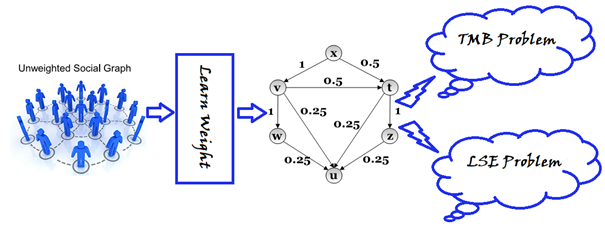
\includegraphics [scale=.5]{picture/Hinh3_1}
		\end{center}
		\caption{Quá trình lấy dữ liệu}
		\label{refhinh3_1}
	\end{figure}
\end{center}
Quá trình lấy dữ liệu, áp dụng để xử lý được mô tả thông qua mô hình ở Hình \ref {refhinh3_1}.
\subsubsection{Thu thập dữ liệu từ MXH Facebook}
Các bước cụ thể của giai đoạn thu thập dữ liệu trên MXH Facebook được mô tả cụ thể như sau:
\begin {itemize}
\item Đầu tiên, nhóm tác giả tạo một tài khoản Facebook rồi sử dụng Công cụ kiểm thử tự động Selenium để tự động đăng nhập vào tài khoản Facebook đó.

\item Bằng các truy vấn đặc biệt, nhóm tác giả lấy được ID (Identity Number) của tài khoản trên.

\item Thông qua phương pháp giám sát và điều tra, thông qua những tin tức, vụ việc trong thời gian gần đây. Nhóm tác giả khảo sát dữ liệu với tập nguồn ban đầu bao gồm 6 tài khoản Facebook, đây là các đối tượng chủ mưu, cầm đầu, nắm vai trò quan trọng trong các tổ chức phản động, thường xuyên có các bài viết, bình luận mang tính chất chống đối, và đặc biệt các đối tượng này có uy tín khá lớn, có lượng người theo dõi, bạn bè trên Facebook là vô cùng đông đảo.
\begin {enumerate} [+]
\item https://www.facebook.com/gioan.namphong: Linh mục giáo sứ Thái Hà Nguyễn Nam Phong, một nhân vật khá nổi tiếng trong làng chống chính quyền trong nước và thường xuyên ra nước ngoài để "liên lạc" với tổ chức khủng bố Việt Tân.

\item https://www.facebook.com/minhnhat.paultran: Paul Trần Minh Nhật là giáo dân thuộc xứ Ngọc Long, xã Công Thành, Yên Thành, Nghệ An, từng bị bắt và kết án 4 năm tù về tội “hoạt động nhằm lật đổ chính quyền nhân dân”. Hiện tại, Minh Nhật đang là cộng tác viên của trang “Tin mừng cho người nghèo”, mang danh nghĩa rao giảng tin mừng của Chúa, nhưng lại nhuốm màu sắc chính trị, luôn ủng hộ các đối tượng vi phạm pháp luật.

\item https://www.facebook.com/ThaiDung2016: Gioan Thái Văn Dung là sinh viên tốt nghiệp ngành tin học, đã tham gia quản lý cửa hàng Internet, Do hiểu biết được CNTT mà biết thêm về xã hội, tích cực truyền bá thông tin, hoạt động mạng, tham gia biểu tình chống TQ xâm lược.

\item https://www.facebook.com/pham.doan.trang: Nhà báo Phạm Đoan Trang, từng công tác tại Báo Pháp Luật thành phố Hồ Chí Minh. Tác giả của cuốn sách “Chính trị Bình Dân” có những nội dung nhạy cảm, mang tính chất kích động, chống phá chính quyền, Đảng và Nhà Nước.

\item https://www.facebook.com/jbnguyenhuuvinh: Anh Ba Sàm, tên thật là Nguyễn Hữu Vinh là một blogger, từng là công an và đảng viên Đảng Cộng sản Việt Nam, từng công tác ở Ủy ban Việt kiều Trung ương. Ông bị Chính phủ CHXHCN Việt Nam bắt giữ và bị cáo buộc và phạt tù 5 năm do có hành vi đăng tải các bài viết trên mạng Internet vi phạm Điều 258 Bộ Luật Hình sự năm 2015 sửa đổi bổ sung năm 2017 về Tội lợi dụng các quyền tự do dân chủ xâm phạm lợi ích của Nhà nước, quyền, lợi ích hợp pháp của tổ chức, công dân.

\item https://www.facebook.com/profile.php?id=100015485029386: Nguyễn Trọng đang sinh sống tại California, Hoa Kỳ. Lợi dụng quyền tự do dân chủ, thường xuyên có những bài viết xuyên tạc, chống phá đường lối chính sác của Đảng, pháp luật của Nhà nước.
\end {enumerate}
\item Tiếp theo, nhóm tác giả tự động trup cập vào trang web có địa chỉ www.facebook.com/{ID}/friends hoặc www.facebook.com/{name}/friends là trang bạn bè của những người dùng đó.

\item Theo thuật toán sắp xếp của Facebook, những người dùng có liên quan nhất và hay tương tác nhất với người dùng đang theo dõi sẽ hiện ra đầu tiên trong trang bạn bè nói trên. Nhóm tác giả sử dụng thư viện BeautifulSoup để lấy mã HTML của trang này, tìm và lấy các đường dẫn chứa địa chỉ Facebook bạn bè của người dùng đang theo dõi, lấy ID của họ.

\item Nhóm tác giả thu thập theo phương pháp loang theo chiều rộng: Bắt đầu từ ID Facebook của 6 đối tượng kể trên, từ đó tìm tiếp thông tin về khoảng 20 người bạn xuất hiện đầu tiên trên trang Facebook bạn bè của mỗi người dùng đó. Với mỗi người dùng thu thập được, nhóm tác giả lại tiếp tục tiến hành thu thập như trên, và cứ tiếp tục tìm kiếm đến khi thu thập đủ số lượng người dùng cần thiết.
\end {itemize}		
Cách làm này có ưu điểm là những người dùng thu thập được có nhiều mối liên hệ với nhau, đồ thị MXH thu thập được có nhiều liên kết, mang lại sự trực quan hơn cho cấu trúc đồ thị mạng. Ngoài ra còn có quá trình tiền xử lý, bước này sẽ hạn chế, loại bỏ được những đỉnh cô lập, hay những đỉnh khai thác được ít thông tin (Không công khai danh sách bạn bè).

Bên cạnh những ưu điểm trên, thì cách làm này cũng có nhược điểm là không khai thác được hết thông tin của người dùng, bởi nhiều người dùng không để chế độ công khai bạn bè. Trong thực tế sẽ để lọt nhiều đối tượng nguy hiểm, ẩn chứa nhiều nguy cơ tiềm tàng.

\subsubsection{Mô hình hóa dữ liệu thu được}
Ở bước này, từ những dữ liệu thu thập được về danh sách ID người dùng, mối quan hệ bạn bè giữa họ. Nhóm tác giả tiền xử lý, đánh số lại các đỉnh, xây dựng đồ thị mô tả MXH với các đỉnh đại diện cho các người dùng, các cạnh biểu diễn mối quan hệ bạn bè giữa những người đó, trọng số (nếu có) đại diện cho mức độ tương tác giữa người dùng với nhau. Kết quả đầu ra của thuật toán thu thập thông tin trên MXH Facebook bao gồm 2 file dữ liệu:
\begin {itemize}
\item ID.txt chứa ánh xạ từ ID của người dùng sang chỉ số đỉnh được đánh số lại. Qua quá trình thu thập dữ liệu, chuẩn hóa, nhóm tác giả thu được 542 ID người dùng, được đánh số lại từ 0 – 541, xem bảng \ref{bang3_1}		
\begin{table} [!htp]
	\centering 
	\begin{tabular}{|c|c|}
		\hline 
		0 & 100003708850657 \\ 
		\hline 
		1 & 100009945675640 \\ 
		\hline 
		2 & 100010197936720 \\ 
		\hline 
		3 & 641613321 \\ 
		\hline 
		4 & 100002541019308 \\ 
		\hline 
		5 & 100015485029386 \\ 
		\hline 
		6 & 100004745583805 \\ 
		\hline 
		... & ... \\ 
		\hline 
		539 & 100004236103486 \\ 
		\hline 
		540 & 100004142778267 \\ 
		\hline 
		541 & 100006259445960 \\ 
		\hline 
	\end{tabular} 
	\caption{Ví dụ ánh xạ ID người dùng sang chỉ số được đánh số.}
	\label{bang3_1}
\end{table}
\item Network.txt chứa mô tả cụ thể của đồ thị MXH đã thu được. File dữ liệu gồm nhiều dòng, mỗi dòng chứa 2 số là chỉ số của 2 người dùng có quan hệ với nhau.

\begin{table} [!htp]
	\centering
	\begin{tabular}{|c|c|}
		\hline 
		0 & 7 \\ 
		\hline 
		0 & 8 \\ 
		\hline 
		0 & 9 \\ 
		\hline 
		0 & 4 \\ 
		\hline 
		... & ... \\ 
		\hline 
		99 & 400 \\ 
		\hline 
		99 & 437 \\ 
		\hline 
		99 & 498 \\ 
		\hline 
	\end{tabular}
	\caption{Mô tả cụ thể của đồ thị MXH thu được}
	\label{bang3_2} 
\end{table}

Từ dữ liệu thu được, nhóm tác giả mô phỏng lại và thu được hình ảnh tổng quan về cấu trúc mạng như sau :

\begin{center}
	\begin{figure}[htp]
		\begin{center}
			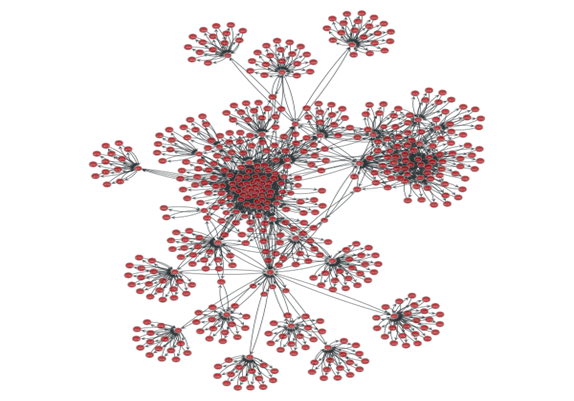
\includegraphics [scale=.5]{picture/Hinh3_2}
		\end{center}
		\caption{Mô phỏng cấu trúc toàn mạng dữ liệu thu được}
		\label{refhinh3_2}
	\end{figure}
\end{center}
\end {itemize}
Trong chương này, nhóm tác giả đưa ra các kết quả thực nghiệm của hai giải pháp đã được đưa ra trong chương trước trên dữ liệu có sẵn và dữ liệu thu thập được, từ đó để thấy được hiệu quả của phương pháp nhóm đề xuất. Dữ liệu có sẵn là các bộ dữ liệu được lấy từ những nguồn uy tín hàng đầu, được các bài báo có chung mục tiêu nghiên cứu khác sử dụng và được các hội nghị, hội thảo thế giới công nhận. Dữ liệu thực là dữ liệu được thu thập trực tiếp trên mạng xã hội Facebook bằng các công cụ thích hợp. Việc sử dụng cả hai loại dữ liệu đảm bảo được rằng các giải pháp đưa ra vừa thỏa mãn được tính chất học thuật cao, vừa thỏa mãn được khả năng ứng dụng thực tế ngay tại Việt Nam.

\section{Giải pháp Limiting the spread of epidemics within time constraint on online social network}
\subsection{Dữ liệu có sẵn}

Trong phần này, chúng tôi thực nghiệm trên một số mạng xã hội trực tuyến để kiểm chứng tính hiệu quả của thuật toán khi so sánh nó với các thuật toán cơ sở được sử dụng trong các bài toán lan truyền thông tin \cite{nguyen30}, \cite{kemple1}, \cite{zhang32}. Chúng tôi so sánh đánh gia trên ba yêu tố chính: chất lượng lời giải, tính mở rộng, tác động của số vòng lan truyền $d$ trên một vài các mạng xã hội trực tuyến thực tiễn. Các thuật toán cơ sở sẽ sử dụng bao gồm:
\begin{itemize}
\item Random: Thuật toán chọn ngẫu nhiên $k$ đỉnh trong $N_{d}(S)$.

\item Maxdegree (Maxdeg): Thuật toán heuristic chọn lần lượt các đỉnh có bậc cao nhất trong tập $V_{d}$ cho đến khi đủ $k$ đỉnh.

\item Greedy: Thuật toán heuristic chọn lần lượt $k$ đỉnh, trong mỗi lần chọn sẽ chọn ra đỉnh sao cho khi loại bỏ đỉnh đó sẽ cứu được nhiều đỉnh nhất có thể.
\end{itemize}

Chúng tôi thực nghiệm sử dụng một hệ thống máy có cấu hình sau: Intel(R) Core(TM) i5-6200U CPU @ 2.30 GHz (up to 2.40 GHz), bộ nhớ RAM 4GB, ngôn ngữ lập trình C++.

\subsubsection{Dữ liêu:}

Chúng tôi thực nghiệm thuật toán trên nhiều bộ dữ liệu thực tế khác nhau. Bên cạnh việc lựa chọn các bộ dữ liệu để đảm bảo sự đa dạng về kích thước, chúng tôi cũng lựa chọn nhiều miền dữ liệu khác nhau, bảng \ref{tab:Table1} thể hiện các bộ dữ liệu nhóm tác giả sử dụng.
\begin{table}
	\centering
	\begin{tabular}{|c|c|c|c|c|}
		\hline 
		Mạng & Số đỉnh & Số cạnh & Loại & Bậc trung bình \\ 
		\hline 
		Gnutella & 6,301 & 20,777 & Có hướng & 3.29 \\ 
		\hline 
		Wikipedia vote & 7,115 & 103,689 & Có hướng & 14.57 \\ 
		\hline 
		Amazon & 262,111 & 1,234,877 & Có hướng & 4.71 \\ 
		\hline 
		Google web & 875,713 & 5,105,039 & Có hướng & 5.83 \\ 
		\hline 
	\end{tabular} 
	\caption{Các bộ dữ liệu}
	\label{tab:Table1}
\end{table}

\subsubsection{Các thiết lập}
Chúng tôi sử dụng các thiết lập dưới đây cho việc đánh giá thực nghiệm:

\begin{itemize}
	\item Trọng số của cạnh: $w(u,v)=\frac{1}{d_{\text{in}}(v)}$, với $d_{\text{in}}(v)$ là bậc vào của đỉnh $v$ \cite{kemple1} \cite{chen10LT} \cite{khali} \cite{amit21}.
	\item Ngưỡng lây nhiễm: chúng tôi lựa chọn ngưỡng lây nhiễm trong tập \\ $\{0.1, 0.2, 0.3, 0.4, 0.5, 0.6, 0.7, 0.8, 0.9\}$.
	\item Số vòng lây nhiễm: chúng tôi lựa chọn số vòng lây nhiễm $d = 2, 3, 4, 5$ dựa theo một nghiên cứu có trước \cite{cha23}.
	\item Số đỉnh bị nhiễm ban đầu: trong mọi bộ dữ liệu, chúng tôi lấy $1\%$ số đỉnh làm tập đỉnh bị lây nhiễm ban đầu. 
\end{itemize}

\subsubsection{Các thuật toán sử dụng}
Chúng tôi sử dụng các thuật toán sau đây cho việc đánh giá thực nghiệm cùng với thuật toán FLE, các thuật toán này đều là các thuật toán được nhiều bài báo khác sử dụng trong quá trình đánh giá của mình:

\begin{itemize}
	\item {\itshape Random}: Thuật toán lựa chọn ngẫu nhiên $k$ đỉnh trong đồ thị mạng xã hội để loại bỏ.
	\item {\itshape Greedy}: Thuật toán thực hiện $k$ lần, mỗi lần chạy thuật toán sẽ thử loại bỏ lần lượt từng đỉnh ra khỏi đồ thị và đánh giá số lượng đỉnh cứu được tuong ứng, qua đó lựa chọn ra đỉnh loại đi mà cứu được nhiều đỉnh nhất để loại bỏ.
	\item {\itshape MaxDegree}: Thuật toán thực hiện $k$ lần, mỗi lần chọn thuật toán sẽ chọn ra đỉnh có bậc lớn nhất để loại nó ra khỏi đồ thị. 
\end{itemize} 

\subsubsection{Kết quả thực nghiệm}

- {\itshape Kết quả lời giải:}

Chúng tôi đo đạc hiệu suất của thuật toán trong ba trường hợp: (1) giá trị $k$ thay đổi từ $10$ đến $100$, $d=5$, $\theta=0.5$ (hình \ref{fig:FLE_k}); (2) ngưỡng $\theta$ thay đổi, $d$ và $k$ giữ nguyên giá trị $50$ (hình \ref{fig:FLE_theta}); (3) giá trị vòng lây nhiêm $d$ thay đổi, $\theta$ và $k$ không đổi (hình \ref{fig:FLE_d}). Trong mọi trường hợp, FLE và Greedy cho kết quả tốt hơn so với các thuật toán còn lại, cụ thể là số lượng đỉnh cứu được nhiều hơn $48.5$ lần so với thuật toán MaxDegree và Random trong hai bộ dữ liệu Gnutella và Wiki Vote. Khi so sánh Greedy và FLE, chúng tôi thấy Greedy có hiệu suất tốt hơn từ $1.02$ đến $1.05$ lần so với FLE trong bộ dữ liệu mạng Gnutella. Tuy nhiên, khoảng cách này bị thu hẹp lại khi $\theta$ và $k$ tăng. Đặc biệt khi $k \geq 50$ và $\theta \geq 0.4$, hiệu suất của hai thuật toán là tương đương nhau. Hình \ref{fig:FLE_k}, \ref{fig:FLE_theta}, \ref{fig:FLE_d} cho thấy Greedy và FLE có hiệu suất tương đương nhau trong bộ dữ liệu mạng Wiki Vote. Trong khi Greedy không thể chạy trong thời gian cho phép trên bộ Amazon và Google Web, FLE vẫn có thể đưa ra kết quả tốt hơn nhiều so với hai thuật toán còn lại.

- {\itshape Kết quả thời gian:}

Thời gian chạy của thuật toán cũng được mô tả trong hình \ref{fig:FLE_k}, \ref{fig:FLE_theta}, \ref{fig:FLE_d}. Đúng như dự đoán, thời gian chạy của Greedy là cực kỳ cao so với các thuật toán còn lại, chiếm $4.5$ phút cho bộ dữ liệu Gnutella và $20.2$ phút cho mạng Wiki Vote. Thuật toán FLE nhanh hơn từ $4820$ đến $6789$ lần so với Greedy trong mạng Gnutella và nhanh hơn từ $5839$ đến $14490$ lần so với Greedy trong mạng Wiki Vote. Điều này xảy ra do Greedy có độ phức tạp thuật toán lớn $O(n_{d}k(m_{d}+n_{d}))$, trong khi FLE chỉ có độ phức tạp nhỏ hơn nhiều $O(k(m_{d}+n_{d}))$. Trong bộ dữ liệu Amazon và Google Web, Greedy không thể tìm thấy lời giải trong vòng $12$ tiếng và bị buộc dừng chạy, trong khi FLE chỉ mất $0.45$ giây và $7.8$ giây tương ứng với mỗi bộ dữ liệu trên. Điều này cho thấy FLE vẫn chạy tốt ngay cả với các bộ dữ liệu lớn.

- {\itshape Ảnh hưởng của tham số $d$:}

Chúng tôi khám phá ảnh hưởng của tham số $d$ đối với các thuật toán khác nhau. Cho $d$ thay đổi từ $2$ đến $5$ trong mạng Gnutella, kết quả được thể hiện trong hình \ref{fig:FLE_d}. Với Greedy và FLE, số đỉnh cứu được tăng khi giá trị $d$ tăng. Đăc biệt, số đỉnh cứu được tăng mạnh với $d=2,3$ và tăng ít hơn với $d=4,5$. Điều này chứng tỏ để ngăn chặn lây lan, ta phải loại bỏ đỉnh càng sớm càng tốt.


- {\itshape Ảnh hưởng của tham số $\theta$:}

Chúng tôi cũng xem xét ảnh hưởng của tham số $\theta$ đối với các thuật toán bằng cách cho $\theta$ thay đổi trong khi giữ nguyên $d$ và $k$. Chúng tôi lựa chọn giá trị $d=5$, $k=50$. Đối với mạng Amazon và Google Web, số đỉnh cứu được sẽ giảm nếu giá trị $\theta$ giảm. Đối với mạng Gnutella và Wiki Vote, số đỉnh cứu được tăng khi $\theta$ tăng từ $0.1$ đến $0.3$ và giảm khi $\theta$ tăng từ $0.3$ đến $0.9$. Tổng quát lại, ta có thể thấy rằng thự tế việc giá trị $\theta$ càng cao sẽ làm quá trình lây làn gặp khó khăn. Từ hình \ref{fig:FLE_theta}, ta thấy Greedy và FLE cho kết quả tốt hơn nhiều so với hai thuật toán còn lại. Điều này một lần nữa cho thấy tính ưu việt của thuật toán FLE.

\begin{figure}
	\begin{tabular}{lll}
		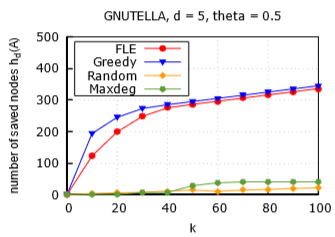
\includegraphics[height = 4.4cm]{picture/FLE/gnu_res} &
		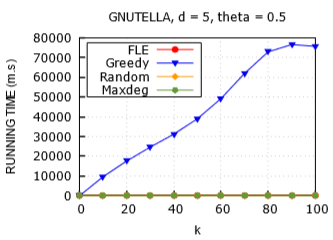
\includegraphics[height = 4.4cm]{picture/FLE/gnu_time} 
		\\
		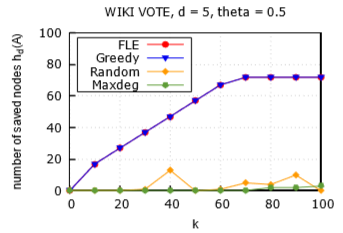
\includegraphics[height = 4.4cm]{picture/FLE/wiki_res} &
		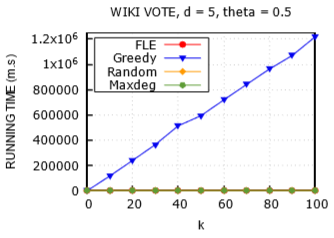
\includegraphics[height = 4.4cm]{picture/FLE/wiki_time} 
		\\
		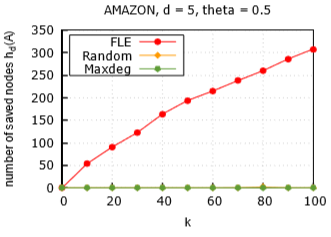
\includegraphics[height = 4.4cm]{picture/FLE/amazon_res} &
		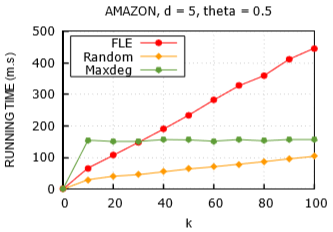
\includegraphics[height = 4.4cm]{picture/FLE/amazon_time} 
		\\
		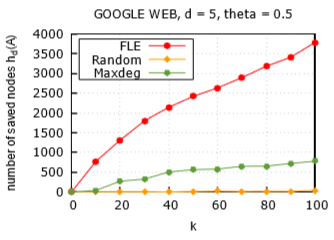
\includegraphics[height = 4.4cm]{picture/FLE/google_res} &
		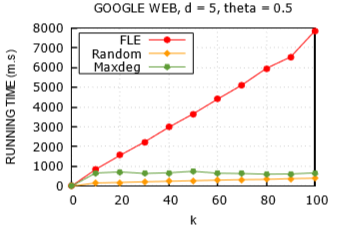
\includegraphics[height = 4.4cm]{picture/FLE/google_time} 
	\end{tabular}
	\caption{So sách chất lượng lời giải và thời gian chạy của các thuật toán khi $k$ thay đổi, $d=5$, $\theta=0.5$.} 
	\label{fig:FLE_k}   
\end{figure}

\begin{figure}
	\begin{tabular}{lll}
		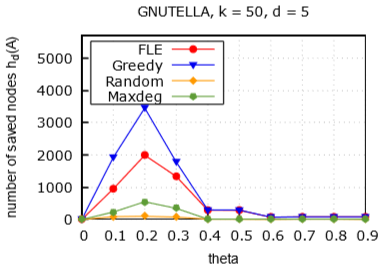
\includegraphics[height = 4.4cm]{picture/FLE/gnu_res_theta} &
		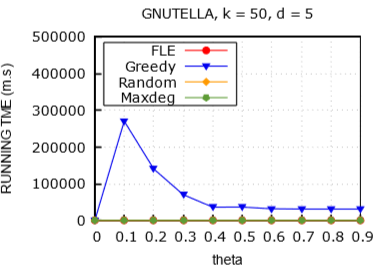
\includegraphics[height = 4.4cm]{picture/FLE/gnu_time_theta} 
		\\
		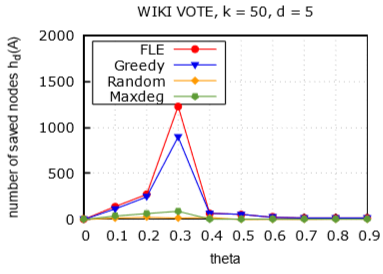
\includegraphics[height = 4.4cm]{picture/FLE/wiki_res_theta} &
		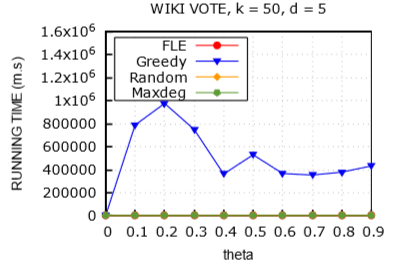
\includegraphics[height = 4.4cm]{picture/FLE/wiki_time_theta} 
		\\
		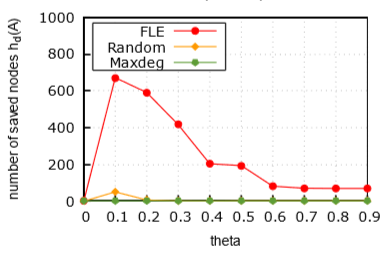
\includegraphics[height = 4.4cm]{picture/FLE/amazon_res_theta} &
		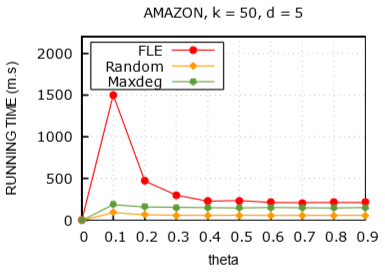
\includegraphics[height = 4.4cm]{picture/FLE/amazon_time_theta} 
		\\
		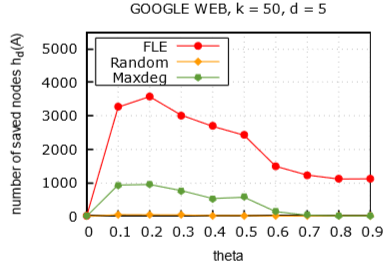
\includegraphics[height = 4.4cm]{picture/FLE/google_res_theta} &
		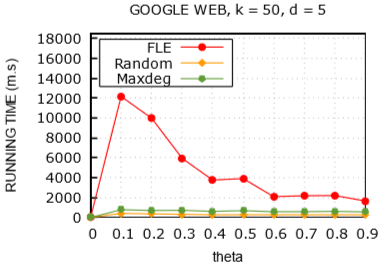
\includegraphics[height = 4.4cm]{picture/FLE/google_time_theta} 
	\end{tabular}
	\caption{So sách chất lượng lời giải và thời gian chạy của các thuật toán khi $\theta$ thay đổi, $d=5$, $k=50$.} 
	\label{fig:FLE_theta}   
\end{figure} 

\begin{figure}
	\begin{tabular}{lll}
		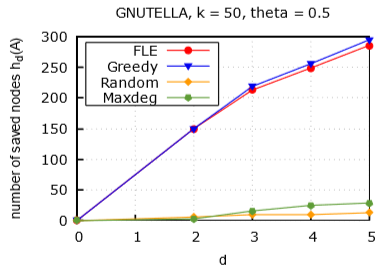
\includegraphics[height = 4.4cm]{picture/FLE/gnu_res_d} &
		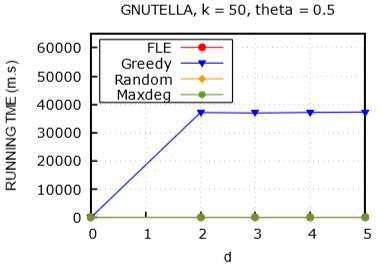
\includegraphics[height = 4.4cm]{picture/FLE/gnu_time_d}
	\end{tabular}
	\caption{So sách chất lượng lời giải và thời gian chạy của các thuật toán khi $d$ thay đổi, $\theta=0.5$, $k=50$ trong mạng Gnutella.} 
	\label{fig:FLE_d}   
\end{figure} 

\section{Giải pháp Targeted Misinformation Blocking (Xác định và ngăn chặn thông tin sai lệch trên mạng xã hội)}
\subsection{Dữ liệu có sẵn}	

Trong mục này chúng tôi đưa ra kết quả thực nghiệm của thuật toán STMB với 3 bộ dữ liệu và so sánh về chất lượng lời giải, tốc độ thực hiện với một số thuật toán cơ bản khác.
\subsubsection{Dữ liệu}
Chúng tôi sử dụng 3 bộ dữ liệu mạng thực tế thu thập trên trang snap.stanford.edu \footnote{https://snap.stanford.edu/data/index.html}, thông tin về chúng được mô tả trong bảng \ref{TMB:table}. 
\begin{table}[h]
	\centering
	\begin{tabular}{|c|c|c|c|}
		\hline 
		Mạng & NetS \cite{NetS} & AS \cite{AS} & NetHEPT \cite{kemple1, chen10LT}\\ 
		\hline 
		Số đỉnh & 1.5K & 6.4K & 15.2K \\ 
		\hline 
		Số cạnh & 5.4K & 12.5K & 32.2K\\ 
		\hline 
		Bậc trung bình & 3.8 & 7.5 & 4.2\\ 
		\hline 
		Số đỉnh nguồn & 100 & 300 & 1000\\ 
		\hline 
	\end{tabular} 
	\caption{Các bộ dữ liệu dùng trong thực nghiệm với giải pháp TMB}
	\label{TMB:table}
\end{table}

Theo các nghiên cứu trước \cite{khali, kemple1,chen10LT}, trọng số các cạnh của đồ thị trên mô hình LT được gán theo công thức $w(u,v) = 1/N_{in}(v)$. Với nguồn phát tán thông tin sai lệch chúng tôi chọn ngẫu nhiên từ 4-6\% số lượng đỉnh của cả đồ thị. Code được viết bằng ngôn ngữ Python 2.7, sử dụng thư viện hỗ trợ NetworkX và chạy trên máy Linux Server với 2.30 GHz Intel\textsuperscript{\textregistered} Xeon\textsuperscript{\textregistered} CPU E5-2697 and 128G of RAM DDR4. Trong thực nghiệm, chúng tôi so sánh thuật toán STMB với một số thuật toán khác được liệt kê dưới đây:
\begin {itemize}
\item PageRank: Tính toán ranking của các đỉnh trong đồ thị G dựa vào cấu trúc các cạnh liên kết với nó. Đây là thuật toán được thiết kế để xếp hạng các trang web từ đó đưa ra kết quả tìm kiếm. Do $h(\cdot)$ là hàm monotone nên sau khi sắp xếp hạng của các đỉnh trong đồ thị, chúng tôi sử dụng thuật toán tìm kiếm nhị phân để tìm kiếm tập lời giải A với |A| đỉnh có rank lớn nhất.
\item High-Degree: Một thuật toán heuristic dựa vào bậc của một đỉnh. Tương tự như thuật toán PageRank sau kho sắp xếp các đỉnh dựa trên bậc của chúng, chúng tôi sử dụng thuật toán tìm kiếm nhị phân để tìm lời giải cho bài toán.
\item Greedy: Thuật toán Greedy đưa ra trong thuật toán \ref{GA} kết hợp với các tối ưu trong \cite{Jleskovec}
\end{itemize} 

\subsubsection{Kết quả thực nghiệm} 
Như mô tả trong hình \ref{solSTMB}, số lượng đỉnh được chọn đưa ra bởi thuật toán STMB là nhỏ nhất. STMB tốt hơn lên đến 39\% so với thuật toán Greedy, hơn 60\%-95\% và 57\%-87\% so với thuật toán PageRank và High-Degree tương ứng. Để kiểm tra kết quả thu được từ thuật toán STMB, chúng tôi chạy 1000 mẫu Monte-Carlo để ước lượng giá trị của hàm $h(A)$ và kết quả kiểm tra được đưa ra trong hình \ref{check}. Trong hầu hết các trường hợp $h(A)$ vượt qua ngưỡng yêu cầu.
\begin{figure}
\begin{tabular}{lll}
	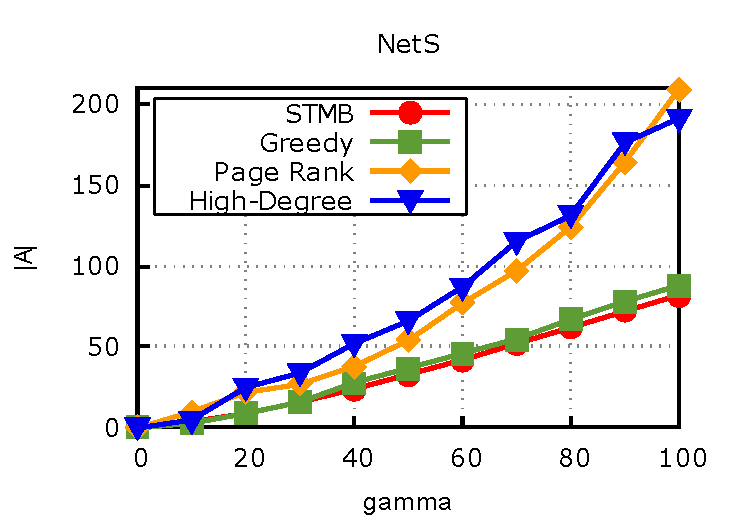
\includegraphics[height = 3.2cm]{picture/NetS} &
	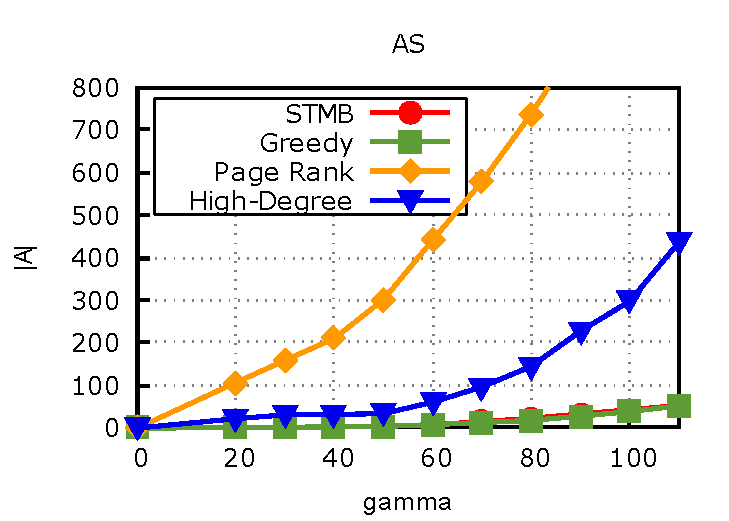
\includegraphics[height = 3.2cm]{picture/AS} &   
	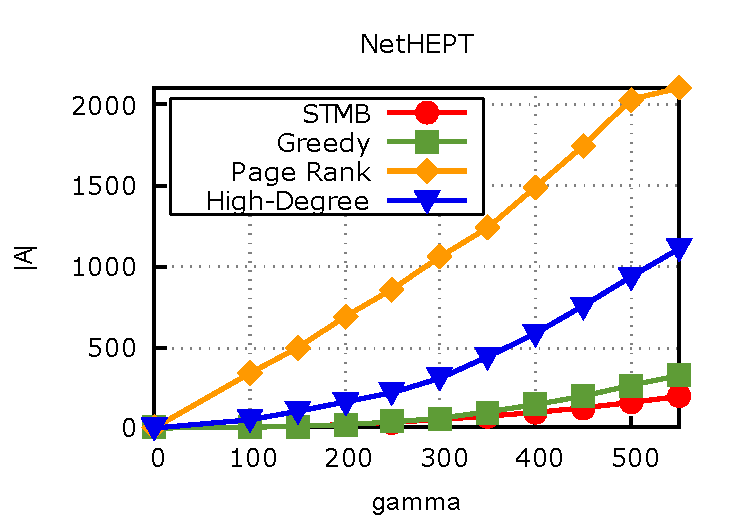
\includegraphics[height = 3.2cm]{picture/NetHEPT}
	\\
	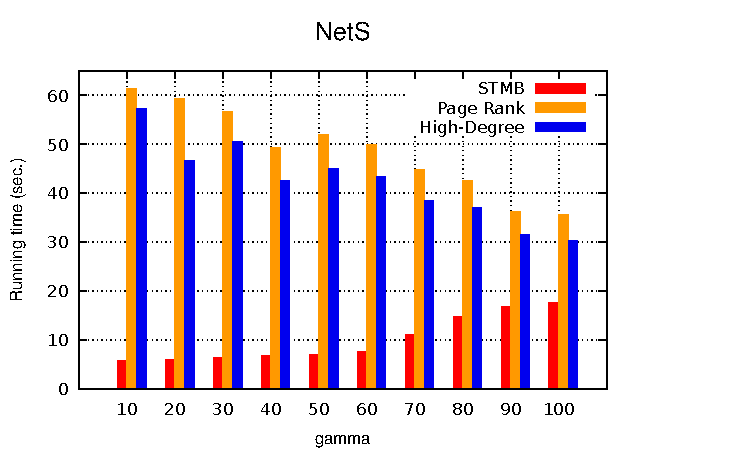
\includegraphics[height = 3.2cm]{picture/TimeNetS} &
	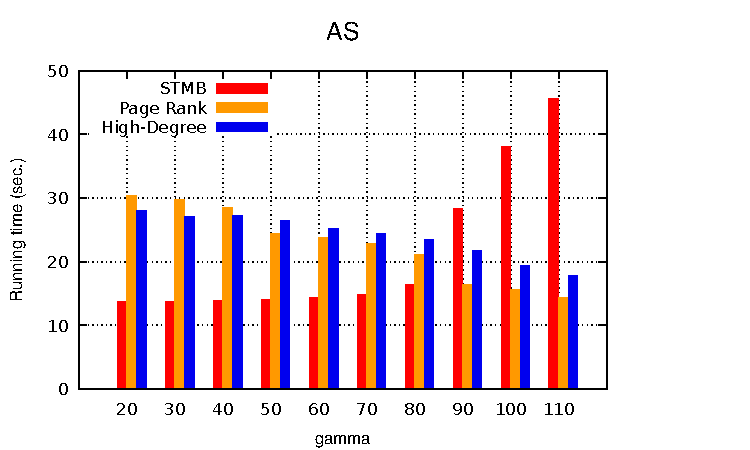
\includegraphics[height = 3.2cm]{picture/TimeAS} &   
	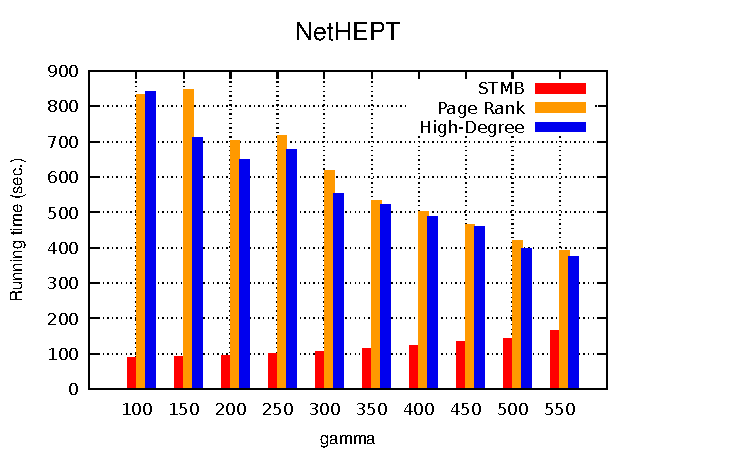
\includegraphics[height = 3.2cm]{picture/TimeNetHEPT}
\end{tabular}
\caption{So sách chất lượng lời giải và thời gian chạy của các thuật toán cho bài toán TMB}
\label{solSTMB}    
\end{figure}
\begin{figure}[htp]
\begin{tabular}{ccc}
	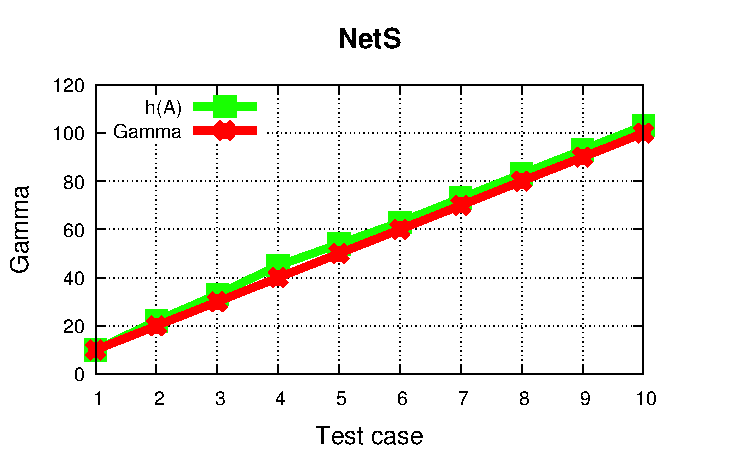
\includegraphics[height = 3.2 cm]{picture/CheckNetS} &
	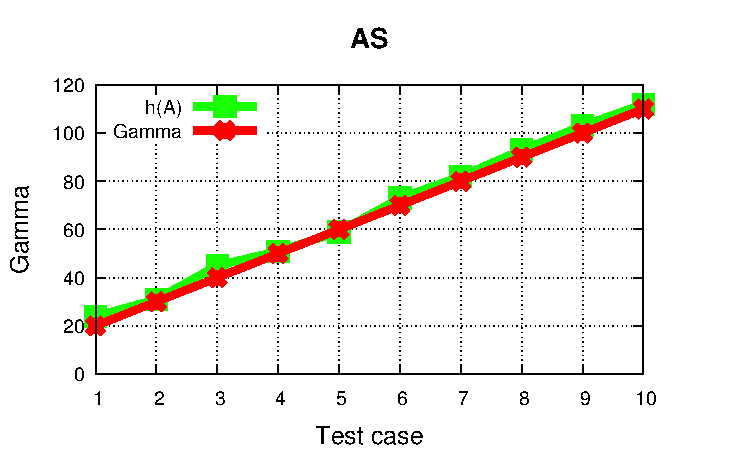
\includegraphics[height = 3.2 cm]{picture/CheckAS} &   
	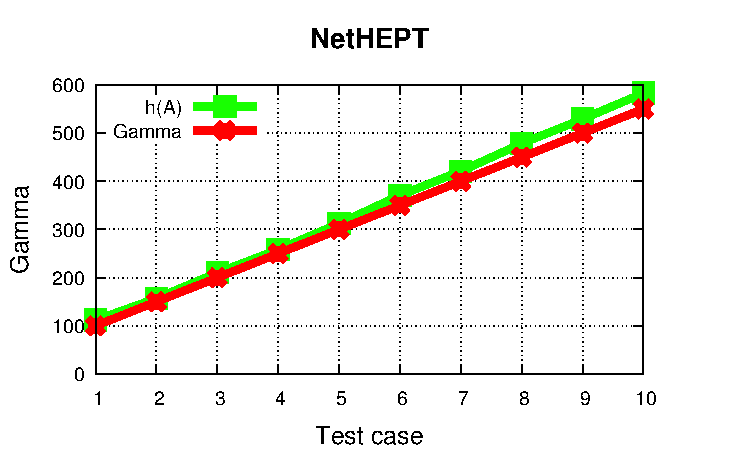
\includegraphics[height = 3.2 cm]{picture/CheckNetHEPT}
\end{tabular}
\caption{Kiểm tra kết quả của thuật toán STMB}
\label{check}    
\end{figure}

Thời gian chạy của các thuật toán trên 3 bộ dữ liệu trong trường hợp có $\gamma$ là lớn nhất được đưa ra trong bảng \ref{timeSTMB}. Ta thấy thuật toán Greedy có chất lượng lời giải tương đương với thuật toán STMB song thời gian thực nghiệm trên các bộ dữ liệu lại rất không hiệu quả.
\begin{table}[h]
\label{tab:time}       % Give a unique label
% For LaTeX tables use
\begin{center}
	\begin{tabular}{|c|c|c|c|c|}				
		\hline 
		\textbf{} & {$\mathsf{STMB}$} & {$\mathsf{Greedy}$} & {Page Rank} & {High-Degree} 				
		\\ 
		\hline 
		NetS & \textbf{17.57(s)} &	14206.80(s) &	35.73(s) &	30.24(s)
		\\ 
		\hline 
		AS & 45.70(s) & 14074.87(s) & \textbf{14.39(s)} &	17.85(s)
		\\
		\hline 
		NetHEPT & \textbf{165.12(s)} & 582566.74(s) & 392.34(s) & 374.66(s)
		\\
		\hline 
	\end{tabular}
\end{center}
\caption{So sánh thời gian chạy của các thuật toán với trường hợp $\gamma$ lớn nhất}
\label{timeSTMB}
\end{table}



